%; whizzy paragraph -pdf xpdf -latex ./whizzypdfptex.sh
%; whizzy-paragraph "^\\\\begin{frame}"
% latex beamer presentation.
% platex, latex-beamer $B$G%3%s%Q%$%k$9$k$3$H$rA[Dj!#(B 

%     Tokyo Debian Meeting resources
%     Copyright (C) 2009 Junichi Uekawa
%     Copyright (C) 2010 Nobuhiro Iwamatsu

%     This program is free software; you can redistribute it and/or modify
%     it under the terms of the GNU General Public License as published by
%     the Free Software Foundation; either version 2 of the License, or
%     (at your option) any later version.

%     This program is distributed in the hope that it will be useful,
%     but WITHOUT ANY WARRANTY; without even the implied warranty of
%     MERCHANTABILITY or FITNESS FOR A PARTICULAR PURPOSE.  See the
%     GNU General Public License for more details.

%     You should have received a copy of the GNU General Public License
%     along with this program; if not, write to the Free Software
%     Foundation, Inc., 51 Franklin St, Fifth Floor, Boston, MA  02110-1301 USA

\documentclass[cjk,dvipdfm,12pt]{beamer}
\usetheme{Tokyo}
\usepackage{monthlypresentation}
%  preview (shell-command (concat "evince " (replace-regexp-in-string "tex$" "pdf"(buffer-file-name)) "&"))
%  presentation (shell-command (concat "xpdf -fullscreen " (replace-regexp-in-string "tex$" "pdf"(buffer-file-name)) "&"))
%  presentation (shell-command (concat "evince " (replace-regexp-in-string "tex$" "pdf"(buffer-file-name)) "&"))
%  presentation (shell-command (concat "evince " (replace-regexp-in-string "tex$" "pdf"(buffer-file-name)) "&"))

%http://www.naney.org/diki/dk/hyperref.html
%$BF|K\8l(BEUC$B7O4D6-$N;~(B
\AtBeginDvi{\special{pdf:tounicode EUC-UCS2}}
%$B%7%U%H(BJIS$B7O4D6-$N;~(B
%\AtBeginDvi{\special{pdf:tounicode 90ms-RKSJ-UCS2}}

\title{$BEl5~%(%j%"(B Debian $BJY6/2q(B}
\subtitle{$B;qNA(B}
\author{$B4d>>(B $B?.MN(B iwamatsu@debian.org\\IRC nick: iwamatsu}
\date{2010$BG/(B04$B7n(B17$BF|(B}
\logo{
\includegraphics[width=8cm]{image200607/openlogo-light.eps}}

\begin{document}

\frame{\titlepage{}}

\emtext{$B@_1D=`Hw$K$46(NO$/$@$5$$(B}

\begin{frame}
 \frametitle{$BJY6/2q$NO"Mm;v9`(B}
\begin{minipage}[t]{0.45\hsize}
  \begin{itemize}
   \item $BCm0U;v9`(B
	 \begin{itemize}
	  \item $B0{?)(B?
	 \end{itemize}
  \end{itemize}
\end{minipage} 
\begin{minipage}[t]{0.45\hsize}
 \begin{itemize}
  \item piuparts $B$N;H$$J}(B
  \item upstart $B:FF~Lg(B
  \item debtags $BF~Lg(B
 \end{itemize}
\end{minipage}
\end{frame}


\begin{frame}
 \frametitle{$BA02s$N(BDebian$BJY6/2q(B}
\begin{minipage}[t]{0.45\hsize}
  \begin{itemize}
   \item $B3t<02q<RD+F|%M%C%H(B 
   \item $BCm0U;v9`(B
         \begin{itemize}
          \item $B0{?)(B?
         \end{itemize}
  \end{itemize}
\end{minipage}
\begin{minipage}[t]{0.45\hsize}
 \begin{itemize}
  \item $B%K%e!<%i%k%M%C%H%o!<%/$G2hA|$rJ,N`$7$F$_$?(B
  \item weka
  \item libfftw
  \item man-db $B?<DI$$(B
  \item dpkg v3 quilt
 \end{itemize}
\end{minipage}
\end{frame}

\begin{frame}{Hack Cafe}
 $B:G6a%O%C%/%+%U%'$7$F$^$9$+(B?\\
 $BKh=5!"?7=I6aJU$G(B Debian Hack Cafe $B$r9T$C$F$$$k$O$:$G$9!#(B\\
 \url{http://twitter.com/debian_hackcafe}\\
\end{frame}

\emtext{$B;vA02]Bj(B}

\begin{frame}{$B;vA02]Bj(B}
\begin{enumerate}
 \item $B9%$-$JF|K\8l(BMan$B%Z!<%8(B
 \item $B%K%e!<%i%k%M%C%H%o!<%/$G2r7h$G$-$kLdBj(B
\end{enumerate}
\end{frame}

{\footnotesize


\begin{prework}{ $B868}=(9/(B }

\begin{enumerate}
\item $B%G%U%)%k%H$N(B2$B$r;HMQ$7$F$$$^$9!#(B
$BDL>o$N%$%s%9%H!<%k$r$7$F$=$N$^$^;HMQ$7$F$$$k$+$i$G$9!#(B
2-5$BA4$FF1$8$J$N$KB>$N%i%s%l%Y%k$r;HMQ$9$k0UL#$O$o$+$C$F$$$^$;$s(B

\item apt-get apptitude$B!"!V%Q%C%1!<%8$NFbMF$r8!:w!W$r;HMQ$7$^$9!#(B
$BL@3N$KL>A0$,J,$+$k$b$N$O(Bapt-get$B$d(Bapptitude$B$G(B
$B$3$&$$$&$b$N$,$[$7$$$H;W$&$H$-$O!V%Q%C%1!<%8$NFbMF$r8!:w!W$r;H$$$^$9!#(B
$B%-!<%o!<%I$,;H$o$l$F$$$J$$%Q%C%1!<%8$G$b8!:w$9$k$3$H$,2DG=$@$+$i$G$9(B
\end{enumerate}

\end{prework}



\begin{prework}{ $B%-%?%O%i(B }
\begin{enumerate}

\item $B%G%U%)%k%H$GAH$_9~$^$l$k!V(Binit$B!W!"FC$KITET9g$,$J$$$?$a!#(B
\item $B:G6a$O!"!V(BGoogle$B@h@8!W$K?R$M$k;v$N$[$&$,B?$$!#(B

\end{enumerate}

\end{prework}



\begin{prework}{ yama1066 }
\begin{enumerate}

\item sysvinit
$B$^$@0\9T$7$F$J$$$+$i!#(B
upstart $B$K0\9T$9$k%a%j%C%H$,5DO@$G$-$l$P$$$$$J$H;W$$$^$9!#(B
\item dselect $B$G$R$?$9$i%4%j%4%j!D!"13$G$9!#(Bapt-cache search $B$G$[$2$[$2!#(B
\end{enumerate}

\end{prework}

\begin{prework}{ henrich }
\begin{enumerate}
\item sysvinit $B$r;H$C$F$^$9!#@N$O(B initng $B$r;H$C$?$3$H$b$"$j$^$7$?$,!D(B
$BLLE]$rHr$1$k$?$a!"$G$9$+$M!#(B
\end{enumerate}

\end{prework}



\begin{prework}{ koedoyoshida }

\begin{enumerate}
\item $B0BDj;V8~$J$N$G(Blenny$BI8=`$N(Binit$B$G$9!#(B
$B;E;v$G;H$C$F$k%^%7%s$O(Bupstart$B$d(Binit$B$,:.:_$7$F$$$^$9!#(B

$B;d$O4pK\E*$K(BLinux$B$O%5!<%P;HMQ$G$9!#(B
$BLGB?$K:F5/F0$7$J$$$N$G$"$^$j287C$r<u$1$F$$$^$;$s!#(B

$BFC$K%a!<%+!<7O$N%5!<%P5!$O(B($B:F(B)$B5/F0;~$K(BSAS,FC$BEy$r4^$a$?(BBIOS$B%A%'%C%/$@$1$G?tJ,$+$+$k$N$b$6$i$J$N$G!"5/F09bB.2=$N%a%j%C%H$O<u$1$K$/$$$H$$$&$N$,@5D>$J$H$3$m$G$9!#(B

init$B0J30$r;HMQ$9$k$3$H$K$h$k!"5/F0;~0J30$N%a%j%C%H$,M-$l$PCN$j$?$$$G$9!#(B

\end{enumerate}

\end{prework}



\begin{prework}{ $BNkLZ?rJ8(B }
\begin{enumerate}
\item sysvinit$B!#(B
$BFC$K%9%T!<%I$r5a$a$h$&$H;W$C$?$3$H$,$J$$$3$H$H!"%5!<%S%95/F0$,HsF14|$@$H2?$+LdBj$,5/$-$?$H$-$KD4::$7$K$/$$%$%a!<%8$,$"$k$?$a!#(B
$B$H$O$$$(!"(BUbuntu$B$N%^%7%s$G$O(BUpstart$B;H$C$F$$$k$N$G!"$?$@N.$5$l$F$$$k$@$1$@$H;W$$$^$9!#(B
\end{enumerate}

\end{prework}



\begin{prework}{ $BF#BtM}Ao(B(risou) }
\begin{enumerate}
\item $B:#;HMQ$7$F$$$k$N$O(B sysvinit $B$G$9!#M}M3$O!"(B lenny $B$N%G%U%)%k%H$K$J$C$F$$$k$+$i$G$9!D!D!#(B
$B!t$3$N$"$?$j!"0c$$$,$h$/$o$+$C$F$J$$$N$G!"$o$6$o$6JQ99$7$F$J$$$G$9!#(B
\end{enumerate}

\end{prework}



\begin{prework}{ $BB<ED?.?M(B }

\begin{enumerate}
\item sysvinit$B!#>/$7A0$K(BSqueeze$B$r%$%s%9%H!<%k$7$?$i%G%U%)%k%H$@$C$?$+$i!#(B
\item  apt-cache search$B$G$6$C$/$j$H8+Ev$r$D$1$F$+$i(Bapt-cache show$B$G>\:Y$r3NG'!#(B
\end{enumerate}
\end{prework}

\begin{prework}{ akedon }

\begin{enumerate}
\item sysvinit $B$G$9!#8=:_!"%G%U%)%k%H$J$N$H%a%+%K%:%`$,C1=c$J$N$G$3$l$GNI$$$+$J$H;W$C$F$$$^$9!#(B
\item aptitude search $B!A(B $B$H(B apt-file search $B!A(B $B$r;H$C$F$$$^$9!#(B
\end{enumerate}
\end{prework}

\begin{prework}{ Hirotaka Kawata }

\begin{enumerate}
\item init$B!#(BDebian $BI8=`$N(B init ($B$U$D$&$N(B init)
\item aptitude search "keyword"
\end{enumerate}
\end{prework}

\begin{prework}{ opentaka }

\begin{enumerate}
\item $B%G%U%)%k%H$N(Binit$B!#%G%U%)%k%H$GF~$C$F$$$?$N$G!#(B
\item aptitude search "package name"
\end{enumerate}
\end{prework}

\begin{prework}{ $B>>_7FsO:(B }
\begin{enumerate}
\item $B$"$^$j0U<1$7$F$$$^$;$s$G$7$?$,!"%G%U%)%k%H$N$b$N$r;H$C$F$$$^$9!#(Bsysvinit?
\item aptitude search hoge
\end{enumerate}
\end{prework}

\begin{prework}{ $B$^$($@$3$&$X$$(B }

\begin{enumerate}
\item sysvinit$B!#%F%9%H4D6-$H$+$G$O(Bupstart$B$b;n$7$F$^$9$,!"(BMacBook$B$N(BSid$B4D6-$H$+$G$O@Z$jBX$($k$N$^$@I]$$$G$9$M!#(B
\item apt-cache
\end{enumerate}
\end{prework}

\begin{prework}{ Yasunori Higashiyama }

\begin{enumerate}
\item sysvinit$B!#FC$K:$$C$F$$$J$$$N$G$=$N$^$^!#(B
\item web$B$G8!:w$+(Baptitude search
\end{enumerate}
\end{prework}

\begin{prework}{ $B4d>>(B $B?.MN(B }

\begin{enumerate}
\item sysvinit $B$G$9!#(BDebian$B$N%G%U%)%k%H$@$+$i$G$9!#(B
\item aptitude $B$G8!:w$7$F$$$^$9(B $B!#%?%0$r;H$$$^$9!#%Q%C%1!<%8$N%$%s%9%H!<(B
      $B%k$O(Bapt $B$G$9$,(B....$B!#$"$H$O!"(Biceweasel$B$d(BGoogle Chrome$B$N8!:w%\%C%/%9$G8!:w$9$k$3$H(B
      $B$b$"$j$^$9!#(B
\end{enumerate}
\end{prework}


\begin{prework}{ google-account@rolf.leggewie.biz }

$B:#2s$b$h$m$7$/$*4j$$$7$^$9!#(B

\end{prework}



}


\section{DWN quiz}
\begin{frame}{Debian $B>o<1%/%$%:(B}

Debian $B$N>o<1!"$b$A$m$sCN$C$F$^$9$h$M(B?
$BCN$i$J$$$J$s$FCQ$:$+$7$/$F!"CN$i$J$$$H$O8@$($J$$$"$s$J$3$H$d$3$s$J$3$H!"(B
$B$_$s$J$G3NG'$7$F$_$^$7$g$&!#(B

$B:#2s$N=PBjHO0O$O(B\url{debian-devel-announce@lists.deban.org} $B$KEj9F$5$l$?(B
$BFbMF$H(BDebian Project News$B$+$i$G$9!#(B

\end{frame}

\subsection{$BLdBj(B}

\santaku
{DPL 2010 $B$KN)8uJd$7$F$$$k$N$OC/!)(B}
{Yasuhiro Araki} % JP 
{Charles Plessy}
{Kurt Roeckx}
{B}

\santaku
{Debian policy 3.8.4.0$B$GDI2C$5$l$?9`L\$O!)(B}
{/sys $B$H(B /selinux $B$N(BFHS$B$KBP$9$kNc30%]%j%7!<(B}
{kFreeBSD$B$H(BLinux$B$r6&B8$9$k%]%j%7!<(B}
{$B%9!<%Q5m$5$s%Q%o!<$K4X$9$k%]%j%7!<(B}
{A}

\santaku
{$B:G6a%O!<%I%&%'%"%H%i%V%k$,$"$C$?%5!<%P$O!)(B}
{rie.debian.org}
{ries.debian.org} % ftp-master.debian.org
{rise.debian.org }
{B}

\santaku
{buildd.debian.org$B$N$"$k%5!<%P$,0\F0$7$^$7$?!#$I$3$K0\F0$7$?$G$7$g$&!#(B}
{peri.debian.org} % ppc buildd
{cimarosa.debian.org} % $B0\F0A0(B
{grieg.debian.org} % $B0\F08e(B
{C}

\santaku
{squeeze$B$N%$%s%9%H!<%i$GDI2C$5$l$?5!G=$O(B}
{Recommends$B$r%$%s%9%H!<%k$9$k$h$&$K$7$^$9(B}
{$B%$%s%9%H!<%i>e$G%Q%C%1!<%8$,%S%k%I$G$-$^$9(B}
{$B%/%m%9%"!<%-%F%/%A%c%$%s%9%H!<%k5!G=$rDI2C$7$^$7$?(B}
{A}

\santaku
{$B?7$7$/(Bmips$BMQ(Bporterbox$B$,DI2C$5$l$^$7$?!#(BCPU$B%3%"?t$O$$$/$D$G$7$g$&$+!#(B}
{64}
{32}
{16}
{C}


% ------------------------------------------------------------------------------
\emtext{piuparts $B$N;H$$J}(B}
% ------------------------------------------------------------------------------

\begin{frame}{$B$O$8$a$K(B}
Piuparts\\
\begin{itemize}
\item $B%$%s%9%H!<%k$N%A%'%C%/(B
\item $B%"%s%$%s%9%H!<%k$N%A%'%C%/(B
\item $B%"%C%W%0%l!<%I$N%A%'%C%/(B
\end{itemize}
\end{frame}


\begin{frame}[containsverbatim]{piuparts$B$N;H$$J}(B}

\begin{itemize}
\item $B%m!<%+%k(BPC$B$K$"$k%Q%C%1!<%8$r%A%'%C%/$9$k(B\\
$B%Q%C%1!<%8%a%s%F%J$,;H$&(B
\item $B4{$K(BDebian$B$K%$%s%9%H!<%k$5$l$F$$$k%Q%C%1!<%8$r%A%'%C%/$9$k(B\\
\texttt{piuparts.debian.org}$B$G;H$&;v$,B?$$(B
\end{itemize}

\end{frame}

\begin{frame}[containsverbatim]{$B<B9T7k2L(B}
\begin{commandline}
$ sudo piuparts libcv4_2.0.0-4_i386.deb -l /tmp/libcv4_2.0.0-4_i386.piuparts-log
0m0.0s INFO: ------------------------------------------------------------------------------
0m0.0s INFO: To quickly glance what went wrong, scroll down to the bottom of this logfile.
0m0.0s INFO: FAQ available at http://wiki.debian.org/piuparts/FAQ
0m0.0s INFO: ------------------------------------------------------------------------------
0m0.0s INFO: piuparts version 0.38 starting up.
0m0.0s INFO: Command line arguments: /usr/sbin/piuparts libcv4_2.0.0-4_i386.deb -l /tmp/libcv4_2.0.0-4_i386.piuparts-log
0m0.0s INFO: Running on: Linux chimagu 2.6.31-1-686 #1
 SMP Sun Nov 15 20:39:33 UTC 2009 i686
0m0.0s DEBUG: Starting command: ['dpkg', '--info', 'libcv4_2.0.0-4_i386.deb']
0m0.2s DUMP:
.... $B>JN,(B .....
6m32.6s DEBUG: Starting command: ['chroot',
 '/tmp/tmplunhrZ', 'umount', '/proc']
6m32.6s DEBUG: Command ok: ['chroot',
 '/tmp/tmplunhrZ', 'umount', '/proc']
6m33.0s DEBUG: Removed directory tree at /tmp/tmplunhrZ
6m33.0s INFO: PASS: All tests.
6m33.0s INFO: piuparts run ends.
\end{commandline}
\end{frame}

\begin{frame}{piuparts$B$NF0:n(B}
\begin{figure}[H]
\begin{center}
\includegraphics[height=0.8\hsize]{image201004/piuparts-process.eps}
\label{fig:piuparts-process}
\end{center}
\end{figure}

\end{frame}

\begin{frame}{$B%m%0$N8+J}(B}

\begin{enumerate}
\item $B%3%^%s%I<B9T(B({\bf DEBUG: Starting command:})
\item $B<B9T3+;O%?%0(B({\bf DUMP:})
\item $B<B9T;~$N%m%0(B
\item $B%3%^%s%I7k2L(B({\bf ERROR:} or {\bf DEBUG: Command ok})
\item $B%F%9%H7k2L(B
\end{enumerate}
\end{frame}


\begin{frame}[containsverbatim]{$B%F%9%H$,@5>o$K=*N;$7$?>l9g(B}

\begin{commandline}
.....$B>JN,(B.....
6m13.7s INFO: PASS: Installation and purging test.
.....$B>JN,(B.....
6m32.6s INFO: PASS: Installation, upgrade and purging tests.
.....$B>JN,(B.....
6m33.0s INFO: PASS: All tests.
6m33.0s INFO: piuparts run ends.
\end{commandline}
\end{frame}

\begin{frame}[containsverbatim]{$B%(%i!<$,$"$k>l9g(B}

\begin{commandline}
0m6.0s DEBUG: Starting command: ['chroot', '/org/piuparts.debian.org/tmp/tmpZ-SX9D', 'apt-get', '-y', 'install', 'upstart']
0m6.3s DUMP:
  Reading package lists...
  Building dependency tree...
  The following extra packages will be installed:
    libdbus-1-3
  Recommended packages:
    dbus
  The following packages will be REMOVED:
    sysvinit
  The following NEW packages will be installed:
    libdbus-1-3 upstart
  WARNING: The following essential packages will be removed.
  This should NOT be done unless you know exactly what you are doing!
    sysvinit
  0 upgraded, 2 newly installed, 1 to remove and 0 not upgraded.
  Need to get 636kB of archives.
  After this operation, 1196kB of additional disk space will be used.
  E: There are problems and -y was used without --force-yes
0m6.3s ERROR: Command failed (status=100): ['chroot', '/org/piuparts.debian.org/tmp/tmpZ-SX9D', 'apt-get', '-y', 'install', 'upstart']
\end{commandline}
\end{frame}

\begin{frame}[containsverbatim]{piuparts$B$N%*%W%7%g%s(B}
$BIaDL$N;H$$J}$G$O;H$$$E$i$$$N$G!"(B\texttt{piuparts}$B$GDs6!$5$l$F$$$k%*%W%7%g%s$r(B
$B<+J,$,;H$C$F$$$k3+H/4D6-$K9g$o$;$F;H$&$N$,IaDL$N$h$&$G$9!#0J2<$G$O(B
$B$h$/;H$&%*%W%7%g%s$r>R2p$7$^$9!#(B
\end{frame}

\begin{frame}[containsverbatim]{pbuilder$B$N(Bbase.tgz$B$r(Bpiuparts$B$GMxMQ$9$k(B}
\begin{commandline}
$ sudo piuparts -p libcv4_2.0.0-4_i386.deb
\end{commandline}
\end{frame}

\begin{frame}[containsverbatim]{$B%G%#%9%H%j%S%e!<%7%g%s$N;XDj(B}
\begin{commandline}
$ sudo piuparts -d sid -d squeeze libcv4_2.0.0-4_i386.deb
.....
\end{commandline}
\end{frame}

\begin{frame}[containsverbatim]{debian$B$K%$%s%9%H!<%k$5$l$F$$$k%Q%C%1!<%8$N%F%9%H(B}
\begin{commandline}
$ sudo piuparts --apt -d squeeze libcv4
\end{commandline}
\end{frame}

\begin{frame}[containsverbatim]{$B%_%i!<%5!<%P$N;XDj(B}

\texttt{--mirror}$B$G;XDj!#(B\\
\begin{commandline}
$ sudo piuparts -p libcv4_2.0.0-4_i386.deb --mirror http://debmirror.example.org/debian
\end{commandline}
\end{frame}

\begin{frame}[containsverbatim]{$B0MB8$9$k%Q%C%1!<%8$N2sHrJ}K!(B}
\begin{itemize}
\item $B%Q%C%1!<%8$N;XDj$G2sHr$9$kJ}K!(B

\begin{commandline}
$ sudo piuparts -p libcv-dev_2.0.0-4_i386.deb libcv4_2.0.0-4_i386.deb
\end{commandline}

\item \texttt{*.changes}$B%U%!%$%k$r;XDj$9$kJ}K!(B

\begin{commandline}
$ sudo piuparts -p opencv_2.0.0-4_i386.changes
\end{commandline}
\end{itemize}
\end{frame}

\begin{frame}[containsverbatim]{piuparts.debian.org}
\begin{itemize}
\item $B%Q%C%1!<%8%a%s%F%J$,%$%s%9%H!<%k!"%"%s%$%s%9%H!<%k!"%"%C%W%0%l!<%I(B
      $B$N%A%'%C%/$7$J$$(B
\item $B%Q%C%1!<%8:n@.;~$O%A%'%C%/$7$?$,!"4D6-$NJQ2=$N$h$k%(%i!<$r%H%i%C%-(B
      $B%s%0$G$-$F$$$J$$(B
\item QA $B%A!<%`$G(B\texttt{piuparts.debian.org}$B$H$7$F%5!<%S%9$rN)$A>e$2$?(B
\end{itemize}
\end{frame}


\begin{frame}[containsverbatim]{$B8=:_%A%'%C%/%(%i!<$K$J$C$F$$$k%Q%C%1!<%8(B}

\begin{itemize}
\item $B%?%0(B : piuparts
\item $B%f!<%6%?%0(B : debian-qa@lists.debian.org
\end{itemize}
$B0J2<$G%A%'%C%/2DG=(B\\
\url{http://bugs.debian.org/cgi-bin/pkgreport.cgi?tag=piuparts;users=debian-qa@lists.debian.org}

\end{frame}

\begin{frame}[containsverbatim]{$B8=:_$NLdBjE@(B}

$B$1$C$3$&0BDj$7$FF0:n$7$F$$$k!#(B

\begin{itemize}
\item $B%A%'%C%/7k2L$,E,@Z$G$O$J$$(B
\item $B%^%K%e%"%kITHw(B\\
\end{itemize}

\begin{commandline}
$ piuparts --help
.... $BCfN,(B ....
 -B FILE, --end-meta=FILE
                     XXX
\end{commandline}

\end{frame}

\begin{frame}[containsverbatim]{$B$^$H$a(B}
\begin{itemize}
\item $B%m%0$O8+$K$/$$$,!"%Q%?!<%s$r8+$l$P$o$+$k!#(B
\item piuparts $B$r%F%9%H%Q%?!<%s$KAH$_9~$_$3$s$G!"%F%9%H$7$^$7$g$&!#(B
\item v2 $B$r3+H/Cf!#3+H/$O(Bbzr$B>e!#(B\\
\url{http://code.liw.fi/piuparts2/bzr/trunk/}
\end{itemize}
\end{frame}


% ------------------------------------------------------------------------------
\emtext{upstart $B:FF~Lg(B}
% ------------------------------------------------------------------------------

% ------------------------------------------------------------------------------
\emtext{debtags $BF~Lg(B}
% ------------------------------------------------------------------------------
\begin{frame}{$B<!2s$NJY6/2q(B}

\begin{itemize}
 \item 2010$BG/(B5$B7n(B21$BF|(B: $BC^GHBg3X(B \\
$BC^GHBg3X(B Linux User Group ($B$D$/$i$0(B) $B$5$s$H9gF13+:E$G$9!#(B

\end{itemize}
 
\end{frame}

\end{document}

;;; Local Variables: ***
;;; outline-regexp: "\\([ 	]*\\\\\\(documentstyle\\|documentclass\\|emtext\\|section\\|begin{frame}\\)\\*?[ 	]*[[{]\\|[]+\\)" ***
;;; End: ***
